\documentclass[12pt,a4paper]{article}
\usepackage{graphicx} % Required for inserting images
\usepackage{tikz}
\usepackage[left=2.00cm, right=1.00cm]{geometry}
\usepackage{xcolor} % before tikz or tkz-euclide if necessary
\usepackage{amsmath}
\usepackage{siunitx}
\usepackage{chemfig}
\title{prøver analysefaget}
\author{Svein-Tore Narvestad}
\date{September 2025}

\begin{document}


\begin{center}
\textbf{Gasslovene:}\\
\end{center}
For ideelle gasser gjelder den ideelle  gasslov:\vspace{1cm}

$$P\cdot V=n\cdot R \cdot T$$ \\\\
der:\\\\
P=gassens trykk (Pa, $N/m^2$)\\
V=Gassens volum ($m^3$)\\
n=Antall mol av gassen, enkelt forklart hvor mange gassmolekyler vi har (mol)\\
R=Gasskonstanten ($\frac{J}{mol\cdot K}$)\\
T=Temperatur (K, $T_K=T_C+273,15$)\\

løst m.h.p. $n\cdot R$:\\\\
$$n\cdot R=\frac{P\cdot V}{T}$$\newpage\noindent 
Her kommer en forklaring på hvorfor vi gjør dette.   Poenget er at uansett hvilken verdi P,V og T har så vil $\frac{P\cdot V}{T}$ være konstant.  La oss se på to eksempler.\\\\
Tilfelle 1:  Her er verdiene $P_1,V_1$ og $T_1$
%sylinder
 \begin{figure}[h]
    \vspace{2cm}  % Flytter figuren ned
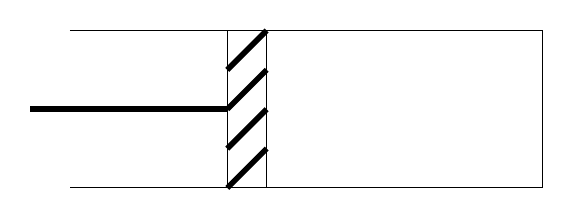
\begin{tikzpicture}
    %stempel med variabel
    \pgfmathsetmacro{\myLength}{4}
    \draw (2,2)--(8,2)--(8,0)--(2,0);
    \draw (\myLength,0)--(\myLength+0.5,0)--(\myLength+0.5,2)--(\myLength,2)--(\myLength,0);
    
    \draw [line width=2pt] (\myLength,0)--(\myLength+0.5,0.5);
    \draw [line width=2pt] (\myLength,0.5)--(\myLength+0.5,1);
    \draw [line width=2pt] (\myLength,1)--(\myLength+0.5,1.5);
    \draw [line width=2pt] (\myLength,1.5)--(\myLength+0.5,2);
    \draw [line width=2pt] (\myLength,1)--(\myLength-2.5,1);
\end{tikzpicture}
\end{figure}\\\\
Tilfelle 2: Her er verdiene $P_2,V_2$ og $T_2$
%sylinder
 \begin{figure}[h]
    \vspace{2cm}  % Flytter figuren ned
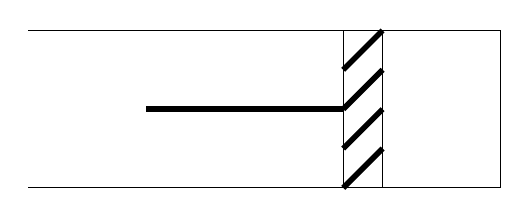
\begin{tikzpicture}
    %stempel med variabel
    \pgfmathsetmacro{\myLength}{6}
    \draw (2,2)--(8,2)--(8,0)--(2,0);
    \draw (\myLength,0)--(\myLength+0.5,0)--(\myLength+0.5,2)--(\myLength,2)--(\myLength,0);
    
    \draw [line width=2pt] (\myLength,0)--(\myLength+0.5,0.5);
    \draw [line width=2pt] (\myLength,0.5)--(\myLength+0.5,1);
    \draw [line width=2pt] (\myLength,1)--(\myLength+0.5,1.5);
    \draw [line width=2pt] (\myLength,1.5)--(\myLength+0.5,2);
    \draw [line width=2pt] (\myLength,1)--(\myLength-2.5,1);
\end{tikzpicture}
\end{figure}\\
Her vil verdiene variere.   Men for begge tilfelle er det slik at:\\\\ 
$n\cdot R=\frac{P_1\cdot V_1}{T_1}$   og $n\cdot R=\frac{P_2\cdot V_2}{T_2}$\\\\
Vi ser at det er likt på venstre side i begge ligningene. Det betyr at:\\

    $$\frac{P_1\cdot V_1}{T_1}=\frac{P_2\cdot V_2}{T_2}$$\\

Denne gjelder for alle P,V og T. Utfra dette kan vi lage noen forenklede lover:\\
Ved konst T:
\begin{center}
    $P_1\cdot V_1=P_2\cdot V_2$
\end{center}
Ved konst P:
\begin{center}
    $\frac{V_1}{T_1}=\frac{V_2}{T_2}$
\end{center}
Ved konstant V:
\begin{center}
    $\frac{P_1}{T_1}=\frac{P_2}{T_2}$
\end{center}
Her kan vi lage oss en enkel huskeregel:
\begin{figure}[h]
    \vspace{2cm}  % Flytter figuren ned
    \centering
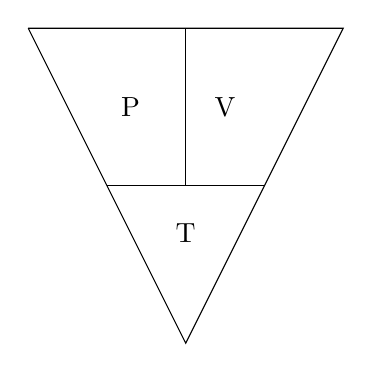
\begin{tikzpicture}
    \draw (4,4)--(6,0)--(8,4)--(4,4);
    \draw (6,4)--(6,2);
    \draw (5,2) -- (7,2);
     \node at (5.3,3) {P};
     \node at (6.5,3) {V};
     \node at (6,1.4) {T};
\end{tikzpicture}
\end{figure}\\
\textbf{Poeng:}Når vi holder over bokstaven for det som er konstant, så vil resten gi oss ligningen.\\\\
Holder vi over T (T=konstant) står det P V altså får vi $P_1\cdot V_1=P_2\cdot V_2$\\
Holder vi over P får vi $\begin{matrix}V\\T\end{matrix}$  altså får vi $\frac{V_1}{T_1}=\frac{V_2}{T_2}$\\
Holder vi over V får vi $\begin{matrix}P\\T\end{matrix}$  altså får vi $\frac{P_1}{T_1}=\frac{P_2}{T_2}$  
\\Ofte må vi snu på disse ligningene, og da kan vi bruke disse enkle kryssene:\\\\
Når T er konstant:
\begin{center}
    \chemfig{(-[:-90]V_1)(-[:0]V_2)(-[:90]P_1)(-[:180]P_2)}
\end{center}\newpage
Når P er konstant:\\
\begin{center}
    \chemfig{(-[:-90]T_2)(-[:0]T_1)(-[:90]V_2)(-[:180]V_1)}
\end{center}
Når V er konstant:\\
\begin{center}
    \chemfig{(-[:-90]T_1)(-[:0]T_2)(-[:90]P_2)(-[:180]P_1)}
\end{center}\newpage\noindent
\textbf{Oppgaver:}\\ %Her begynner oppgavene
\begin{enumerate}
    \item Regn om til Kelvin grader: $-25^0C\quad 0^0C \quad 50^0C \quad 100^0C$
    \item Hvilke enheter bruker vi for trykk (P), volum (V) og temperatur (T) i disse formlene?
    \item Hvordan er Kelvin temperaturen definert?
    \item Vi har gitt følgende system der $P_1=1bar,
    \\ T_1=25^0C$.\quad Volumet er 6,3L:
     \begin{figure}[h]
    \vspace{2cm}  % Flytter figuren ned
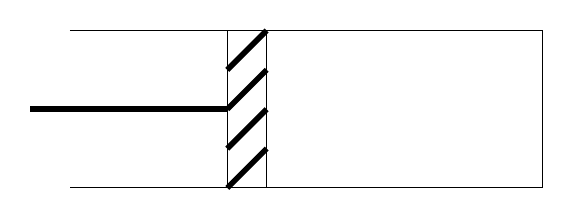
\begin{tikzpicture}
    %stempel med variabel
    \pgfmathsetmacro{\myLength}{4}
    \draw (2,2)--(8,2)--(8,0)--(2,0);
    \draw (\myLength,0)--(\myLength+0.5,0)--(\myLength+0.5,2)--(\myLength,2)--(\myLength,0);
    
    \draw [line width=2pt] (\myLength,0)--(\myLength+0.5,0.5);
    \draw [line width=2pt] (\myLength,0.5)--(\myLength+0.5,1);
    \draw [line width=2pt] (\myLength,1)--(\myLength+0.5,1.5);
    \draw [line width=2pt] (\myLength,1.5)--(\myLength+0.5,2);
    \draw [line width=2pt] (\myLength,1)--(\myLength-2.5,1);
\end{tikzpicture}
\end{figure}\\\\
a) Hva blir trykket om vi endrer volumet til 3,6L når temperaturen er konstant?\\
b) Hva blir trykket om vi endrer temperaturen til $83^0C$ og holder volumet konstant
lik 3,6L?\\\\
\noindent
5. En gass er innestengt i en beholder:
     \begin{figure}[h]
    \vspace{1cm}  % Flytter figuren ned
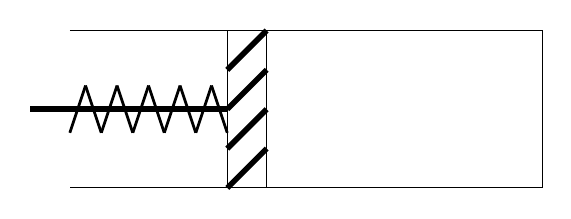
\begin{tikzpicture}
    %stempel med variabel
    \pgfmathsetmacro{\myLength}{4}
    \draw (2,2)--(8,2)--(8,0)--(2,0);
    \draw (\myLength,0)--(\myLength+0.5,0)--(\myLength+0.5,2)--(\myLength,2)--(\myLength,0);
    
    \draw [line width=2pt] (\myLength,0)--(\myLength+0.5,0.5);
    \draw [line width=2pt] (\myLength,0.5)--(\myLength+0.5,1);
    \draw [line width=2pt] (\myLength,1)--(\myLength+0.5,1.5);
    \draw [line width=2pt] (\myLength,1.5)--(\myLength+0.5,2);
    \draw [line width=2pt] (\myLength,1)--(\myLength-2.5,1);
    \draw [line width=1pt] (2,0.7)--(2.2,1.3);
    \draw [line width=1pt] (2.2,1.3)--(2.4,0.7);
    \draw [line width=1pt] (2.4,0.7)--(2.6,1.3);
    \draw [line width=1pt] (2.6,1.3)--(2.8,0.7);
    \draw [line width=1pt] (2.8,0.7)--(3.0,1.3);
    \draw [line width=1pt] (3.0,1.3)--(3.2,0.7);
    \draw [line width=1pt] (3.2,0.7)--(3.4,1.3);
    \draw [line width=1pt] (3.4,1.3)--(3.6,0.7);
    \draw [line width=1pt] (3.6,0.7)--(3.8,1.3);
    \draw [line width=1pt] (3.8,1.3)--(4.0,0.7);
\end{tikzpicture}
\end{figure}\\\\
Trykket inne i beholderen er 5bar, volumet er 3,8L og temperaturen er $123^0C$.  Denne sylinderen er en slags sikkerhetsventil.  Her er det påmontert en fjær som gjør at når trykket er over 8bar så vil stempelet bevege seg utover. Gassen i beholderen skal varmes opp.\\
a) Ved hvilken temperatur vil sikkerhetsventilen utløses?\\\\
b) Hvor stor er kraften mot stempelet når stempelets radius er 7,3cm? Hint: $P=\frac{F}{A}$?\\\\
c) Stempelet beveger seg utover til trykket i gjen er 5bar.  Temperaturen er konstant.  Hva blir det nye volumet?\\\\
d) Hvor langt har stempelet flyttet seg?
\end{enumerate}\vspace{1cm}
\textbf{Svar på oppgaver:}\\
1) Regn om til kelvin grader: $-25^0C\quad 0^0C \quad 50^0C \quad 100^0C$: \\
Formelen for omregning fra celisus til kelvin:  $T_K=T_C+273,15$\\
For $-25^0C: -25+273,15=248,15K$\\
For $0^0C: 0+273,15=273,15K$\\
For $50^0C: 50+273,15=323,15K$\\
For $100^0C: 100+273,15=373,15K$\\\\
2) Hvilke enheter bruker vi for trykk (P), volum (V) og temperatur (T) i disse formlene?\\
Svar: Vi skal bruke SI enhetene for trykk, temperatur og volum.  \\\\
Definisjon på trykk: $P=\frac{F}{A}$ \\
der:\\
F=kraft (N)\\
A=areal ($m^2$)\\
P=trykk ($N/m^2)$ Denne enheten kalles for Pa (Pascal). Mer vanlig enhet for trykk er bar.  Her gjelder følgende: $P_{Pa} = 10^5\cdot P_{bar}$  NB! $10^5=10\cdot 10\cdot 10\cdot 10\cdot10=100000$\\
Viktig å vite når det gjelder gasslover: Vi kan bruke hva som helst for P og V, men T må være i Kelvin. \\\\
3) Hvordan er Kelvin temperaturen definert?\\
\textbf{Svar:} Lord Kelvin kom frem til at den laveste mulige temperaturen er $-273,15^0C$.  han valgte derfor sin egen skala slik at $0K=-273,15^0C$.  Vi finner temperaturen i Kelvin ved å plusse på 273,15.\newpage\noindent
4) Vi har gitt følgende system der $P_1=1bar,
    \\ T_1=25^0C$.\quad Volumet er 6,3L:
     \begin{figure}[h]
    \vspace{2cm}  % Flytter figuren ned
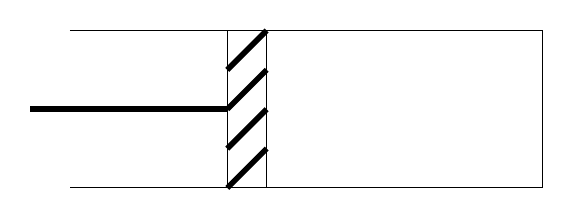
\begin{tikzpicture}
    %stempel med variabel
    \pgfmathsetmacro{\myLength}{4}
    \draw (2,2)--(8,2)--(8,0)--(2,0);
    \draw (\myLength,0)--(\myLength+0.5,0)--(\myLength+0.5,2)--(\myLength,2)--(\myLength,0);
    
    \draw [line width=2pt] (\myLength,0)--(\myLength+0.5,0.5);
    \draw [line width=2pt] (\myLength,0.5)--(\myLength+0.5,1);
    \draw [line width=2pt] (\myLength,1)--(\myLength+0.5,1.5);
    \draw [line width=2pt] (\myLength,1.5)--(\myLength+0.5,2);
    \draw [line width=2pt] (\myLength,1)--(\myLength-2.5,1);
\end{tikzpicture}
\end{figure}\\

\noindent a) Hva blir trykket om vi endrer volumet til 3,6L når temperaturen er konstant?\\\\
\textbf{Svar:} Siden temperaturen er konstant så bruker vi Boyles lov:\\\\
    $$P_1\cdot V_1=P_2 \cdot V_2$$

Vi løser m.h.p. $P_2$ :
\begin{center}
    $P_2=\frac{P_1\cdot V_1}{V_2}$
\end{center}
Vi setter inn verdier:\\

    $$P_2=\frac{1bar\cdot 6,3L}{3,6L}=1,75bar$$\\

\noindent b) Hva blir trykket om vi endrer temperaturen til $83^0C$ og holder volumet konstant?\\
Siden Volumet er konstant bruker vi Gay-Lussacs lov:

    $$\frac{P_3}{T_3}=\frac{P_2}{T_2}$$

Løst m.h.p. $P_3$: 
$$P_3=\frac{P_2\cdot T_3}{T_2}$$\\
Vi setter inn verdier:\\
$$P_3=\frac{P_2\cdot T_3}{T_2}=\frac{1,75bar \cdot (83+273,15)K}{298,15K}=2,09bar$$\newpage\noindent
5. En gass er innestengt i en beholder:
     \begin{figure}[h]
    \vspace{1cm}  % Flytter figuren ned
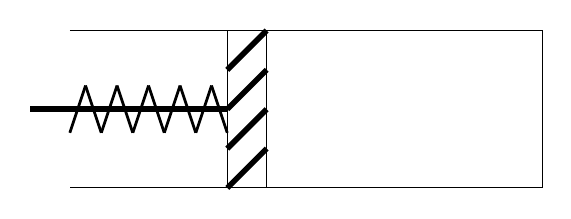
\begin{tikzpicture}
    %stempel med variabel
    \pgfmathsetmacro{\myLength}{4}
    \draw (2,2)--(8,2)--(8,0)--(2,0);
    \draw (\myLength,0)--(\myLength+0.5,0)--(\myLength+0.5,2)--(\myLength,2)--(\myLength,0);
    
    \draw [line width=2pt] (\myLength,0)--(\myLength+0.5,0.5);
    \draw [line width=2pt] (\myLength,0.5)--(\myLength+0.5,1);
    \draw [line width=2pt] (\myLength,1)--(\myLength+0.5,1.5);
    \draw [line width=2pt] (\myLength,1.5)--(\myLength+0.5,2);
    \draw [line width=2pt] (\myLength,1)--(\myLength-2.5,1);
    \draw [line width=1pt] (2,0.7)--(2.2,1.3);
    \draw [line width=1pt] (2.2,1.3)--(2.4,0.7);
    \draw [line width=1pt] (2.4,0.7)--(2.6,1.3);
    \draw [line width=1pt] (2.6,1.3)--(2.8,0.7);
    \draw [line width=1pt] (2.8,0.7)--(3.0,1.3);
    \draw [line width=1pt] (3.0,1.3)--(3.2,0.7);
    \draw [line width=1pt] (3.2,0.7)--(3.4,1.3);
    \draw [line width=1pt] (3.4,1.3)--(3.6,0.7);
    \draw [line width=1pt] (3.6,0.7)--(3.8,1.3);
    \draw [line width=1pt] (3.8,1.3)--(4.0,0.7);
\end{tikzpicture}
\end{figure}
\\\\Trykket inne i beholderen er 5bar, volumet er 3,8L og temperaturen er $123^0C$.  Denne sylinderen er en slags sikkerhetsventil.  Her er det påmontert en fjær som gjør at når trykket er over 8bar så vil stempelet bevege seg utover. Gassen i beholderen skal varmes opp.\\\\
a) Ved hvilken temperatur vil sikkerhetsventilen utløses?\\\\
Sikkerhetsventilen vil utløses når trykket er 8bar.  Vi antar at volumet ikke endrer seg, og  dermed kan vi bruke loven om konstant volum (Guy Lussacs lov):\\
$$\frac{P_2}{T_2}=\frac{P_1}{T_1}$$\\
Vi løser dette m.h.p. $T_2:$\\\\
$$T_2=\frac{P_2\cdot T_1}{P_1}=\frac{8bar\cdot (123+273,15)K}{5bar}=633,84K$$\\
I celsius:  $(633,84-273,15)^oC=360,69^oC$\\\\
b) Hvor stor er kraften mot stempelet når stempelets radius er 7,3cm? Hint: $P=\frac{F}{A}$?\\\\
Denne oppgaven krever at man forstår hva trykk egentlig er. definisjonen på trykk er $P=\frac{F}{A}$.  Altså hvor mye kraft det er pr. areal.  Nå skal vi se på kraften mot stempelet.  Formelen blir: $F=P\cdot A$. Vi må derfor beregne arealet av stempelet.  Det tenker vi oss er en sirkel med radius 7,3cm.  Siden vi jobber med SI enheter må vi gjøre om til meter: r=0,073m.  Arealet til sirkelen blir:\\
$$A=\pi\cdot r^2=3,14\cdot 0,073\cdot0,073m^2=0,0167m^2$$\\
Formelen for kraften er $F=P\cdot A$  Men vi må da gjøre om trykket til Pascal, eller $N/m^2$.  Det får vi ved å "gange" med 100000.  Så 1 bar =100000Pa. Dermed blir 8bar =800000Pa.\\
Kraften blir:\\
$$F=P\cdot A=800000Pa\cdot 0,0167m^2=13360N$$\\\\
c) Stempelet beveger seg utover til trykket i gjen er 5bar.  Temperaturen er konstant.  Hva blir det nye volumet?\\\\
Temperaturen er konstant, og da gjelder Boyles lov:\\
$$P_1\cdot V_1=P_2\cdot V_2$$\\
Løst m.h.p. $V_2$:\\
$$V_2=\frac{P_1\cdot V_1}{P_2}=\frac{8bar\cdot3,8L}{5bar}=6,08L$$ \newpage
d) Hvor langt har stempelet flyttet seg?\\
Her må vi se litt på hva som skjer.  Vi starter med et volum $V_1=3,8L$:\vspace{1.5cm}

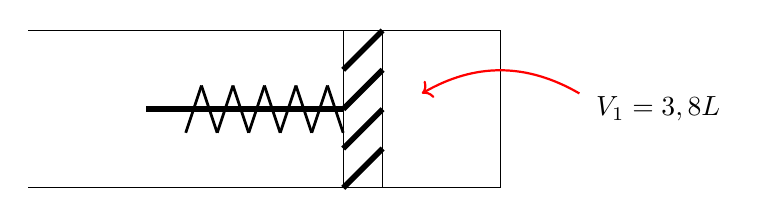
\begin{tikzpicture}
    %stempel med variabel
    \pgfmathsetmacro{\myLength}{6}
    \pgfmathsetmacro{\feather}{\myLength-4}
    \draw (2,2)--(8,2)--(8,0)--(2,0);
    \draw (\myLength,0)--(\myLength+0.5,0)--(\myLength+0.5,2)--(\myLength,2)--(\myLength,0);
    
    \draw [line width=2pt] (\myLength,0)--(\myLength+0.5,0.5);
    \draw [line width=2pt] (\myLength,0.5)--(\myLength+0.5,1);
    \draw [line width=2pt] (\myLength,1)--(\myLength+0.5,1.5);
    \draw [line width=2pt] (\myLength,1.5)--(\myLength+0.5,2);
    \draw [line width=2pt] (\myLength,1)--(\myLength-2.5,1);
    \draw [line width=1pt] (\feather+2,0.7)--(\feather+2.2,1.3);
    \draw [line width=1pt] (\feather+2.2,1.3)--(\feather+2.4,0.7);
    \draw [line width=1pt] (\feather+2.4,0.7)--(\feather+2.6,1.3);
    \draw [line width=1pt] (\feather+2.6,1.3)--(\feather+2.8,0.7);
    \draw [line width=1pt] (\feather+2.8,0.7)--(\feather+3.0,1.3);
    \draw [line width=1pt] (\feather+3.0,1.3)--(\feather+3.2,0.7);
    \draw [line width=1pt] (\feather+3.2,0.7)--(\feather+3.4,1.3);
    \draw [line width=1pt] (\feather+3.4,1.3)--(\feather+3.6,0.7);
    \draw [line width=1pt] (\feather+3.6,0.7)--(\feather+3.8,1.3);
    \draw [line width=1pt] (\feather+3.8,1.3)--(\feather+4.0,0.7);
    \node at (10,1) {$V_1=3,8L$};
    \draw[<-, bend left,red,thick] (7,1.2) to (9,1.2);
\end{tikzpicture}\\\\
Så varmer vi opp, og trykket øker. Når trykket har blitt 8bar klarer ikke fjæren å holde på stempelet lenger så det beveger seg utover, og det stopper når trykket er 5bar.  Volumet har da blitt 6,08L:\vspace{1.5cm}

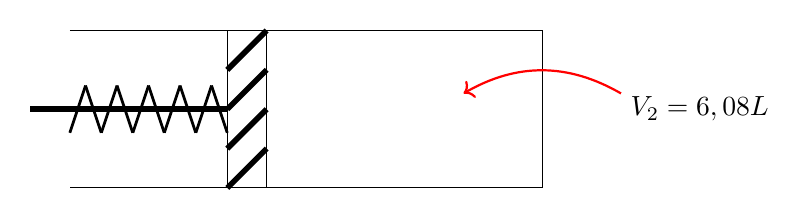
\begin{tikzpicture}
    %stempel med variabel
    \pgfmathsetmacro{\myLength}{4}
    \pgfmathsetmacro{\feather}{\myLength-4}
    \draw (2,2)--(8,2)--(8,0)--(2,0);
    \draw (\myLength,0)--(\myLength+0.5,0)--(\myLength+0.5,2)--(\myLength,2)--(\myLength,0);
    \draw [line width=2pt] (\myLength,0)--(\myLength+0.5,0.5);
    \draw [line width=2pt] (\myLength,0.5)--(\myLength+0.5,1);
    \draw [line width=2pt] (\myLength,1)--(\myLength+0.5,1.5);
    \draw [line width=2pt] (\myLength,1.5)--(\myLength+0.5,2);
    \draw [line width=2pt] (\myLength,1)--(\myLength-2.5,1);
    \draw [line width=1pt] (\feather+2,0.7)--(\feather+2.2,1.3);
    \draw [line width=1pt] (\feather+2.2,1.3)--(\feather+2.4,0.7);
    \draw [line width=1pt] (\feather+2.4,0.7)--(\feather+2.6,1.3);
    \draw [line width=1pt] (\feather+2.6,1.3)--(\feather+2.8,0.7);
    \draw [line width=1pt] (\feather+2.8,0.7)--(\feather+3.0,1.3);
    \draw [line width=1pt] (\feather+3.0,1.3)--(\feather+3.2,0.7);
    \draw [line width=1pt] (\feather+3.2,0.7)--(\feather+3.4,1.3);
    \draw [line width=1pt] (\feather+3.4,1.3)--(\feather+3.6,0.7);
    \draw [line width=1pt] (\feather+3.6,0.7)--(\feather+3.8,1.3);
    \draw [line width=1pt] (\feather+3.8,1.3)--(\feather+4.0,0.7);
    \node at (10,1) {$V_2=6,08L$};
    \draw[<-, bend left,red,thick] (7,1.2) to (9,1.2);
\end{tikzpicture}\\\\
Vi ser at endringen i volum er lik $V_2-V_1=6,08L-3,8L=2,28L.$ Dette volumet kan tegnes som en sylinder:\\\\\\
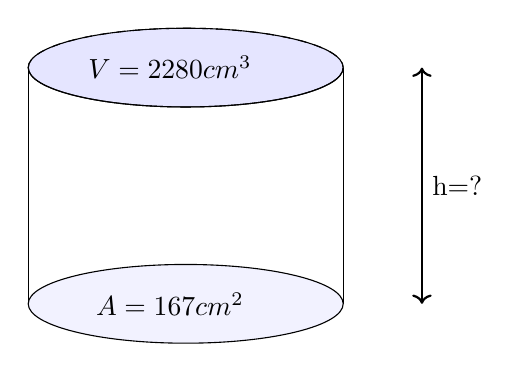
\begin{tikzpicture}
 % Øverste ellipse (synlig topp)
  \draw[fill=blue!10] (2,0) ellipse (2 and 0.5);
  % Sylinderens vegger
  \draw (0,0) -- (0,-3);
  \draw (4,0) -- (4,-3);

  % Bunn (delvis skjult ellipse)
  \draw[fill=blue!5] (2,-3) ellipse (2 and 0.5);

  % Topp (foran) ellipsebue
  \draw (0,0) arc[start angle=180, end angle=360, x radius=2, y radius=0.5];

  % Bunn (bak) ellipsebue (stiplet, fordi den er skjult)
  \draw[dashed] (0,0) arc[start angle=180, end angle=0, x radius=2, y radius=0.5];
  \node at (1.8,-3) {$A=167cm^2$};
  \node at (1.8,0) {$V=2280cm^3$};
  \draw[<->, thick] (5,0) to node[right]{h=?} (5,-3);
\end{tikzpicture}\vspace{1cm}\\
Her trengs det litt forklaring:  I dette tilfellet er det enklest å jobbe cm. Vi gjør derfor om volumet om til milliliter (mL) som er lik $cm^3$: $2,28L=2280mL=2280cm^3$.  Arealet har vi regnet til $0,0167m^2$ som er lik $167cm^2$.  Dette kan vi også beregne:\\
$$ A =\pi\cdot r^2=3,14\cdot 7,3cm \cdot 7,3cm=167$$\newpage 
\noindent For volumet kan vi skrive at:\\
$$V=A\cdot h$$\\
Løst m.h.p. h:\\
$$h=\frac{V}{A}=\frac{2280cm^3}{167cm^2}=13,7cm$$\\
Stempelet vil altså flytte seg 13,7cm utover.
\end{document}
 